% -*- root: ../main.tex -*-

% Esporre i principali problemi affrontati durante l'effettiva realizzazione delle componenti hardware/software e illustrare le soluzioni implementative adottate. Se l'elaborato ha previsto l'utilizzo di tecnologie già disponibili sul mercato, discuterne brevemente le caratteristiche e motivarne l'adozione rispetto ad altre soluzioni assimilabili. NOTA: in questa sezione devono essere riportate esclusivamente le porzioni di codice ritenute particolarmente significative.
% 10000 - 21000 battute

\chapter{Implementazione}
\section{Microcontrollori}
\subsection{Battito Cardiaco}
Un parte particolarmente complessa è stata quella della modellazione del sensore per il battito. Il sensore, qualora interpellato, fornisce un singolo valore direttamente proporzionale alla dilatazione dei vasi sanguigni. Ne deriva la necessità di attuare misurazioni frequenti per non incorrere nella perdita della breve variazione di un battito. Abbiamo stabilito la frequenza di campionamento in base a quanto segue:
Considerando che in condizioni di riposo, i battiti per minuto di un cane - da intendersi come pulsazioni - sono generalmente compresi tra 60 e 140 bpm, in base alla taglia, età e razza, e il valore può raggiungere valori anche più alti qualora in movimento, abbiamo preso come valore limite da rilevare 150 bpm. Ciò, significa che il tempo di ogni ciclo cardiaco $T_{cc}$ è:
\begin{equation}
T_{cc} = \frac{1}{bps} = \frac{1}{\frac{bpm}{60}}= \frac{60}{bpm} \Rightarrow \frac{60}{150 bpm} = 0.4s
\end{equation}
Considerato che il ciclo cardiaco si compone in sistole (contrazione) e diastole (rilassamento), la fase sistolica è quella più facilmente rilevabile poiché la contrazione ventricolare causata è più violenta e breve. Questa fase durante le rilevazioni effettuate dura circa un mezzo del ciclo cardiaco e produce un picco nei valori particolarmente indicativo per rilevare il battito in mezzo al naturale rumore del sensore. Per non perdere il picco massimo il numero di campionamenti $N_{c}$ durante questa fase è stato fissato a 20. La frequenza di campionamento minima risultante $f_{min}$ è stata calcolata come: 
\begin{equation}
f_{min} = \frac{ \frac{1}{2} *  T_{cc} }{N_{c}} \Rightarrow  \frac{ \frac{1}{2} *  0.4s }{20} = 0.01s = 10 ms 
\end{equation}

Salvando i valori risultanti e graficandoli con la libreria python "Mathplotlib" si ottiene una linea come quella di colore rosso in [Fig. \ref{fig:Heartbeat}]. Si può notare che il campionamento è sufficiente e permette di distinguere intuitivamente i battiti. 
Per rilevare le pulsazioni a livello digitale però è necessario formalizzare un altro modello matematico che non faccia incorrere il sistema in falsi positivi o falsi negativi. Un primo approccio si è basato su stabilire una singola soglia, oltre la quale il battito è rilevato e registrato. Questa soluzione si è rivelata inadatta in quanto il disturbo del sensore la farebbe attraversare più volte (si veda in [Fig. \ref{fig:Heartbeat}] poco prima del campionamento numero 2400 il valore attraversa la linea azzurra parecchie volte). Inadatti si sono rivelati anche i tentativi di normalizzare la linea dei valori, in quanto parecchio discontinui e di frequenza elevata, si perde la differenziazione dei picchi. Si è optato per stabilire una doppia soglia, la prima, più alta, oltre la quale il battito è rilevato, la seconda, più bassa, che determina la fine del battito. La prima volta che il valore attraversa la prima [Fig. \ref{fig:Heartbeat}, linea azzurra] una variabile registra il battito e nessun altra registrazione viene effettuata sino a che i valori non scendono sotto la soglia di fine battito [Fig. \ref{fig:Heartbeat}, linea gialla]. 
Queste soglie non possono essere fisse, variando la pressione di animale in animale e pure di giorno in giorno per lo stesso essere vivente. Per questo motivo i valori sono stati fissati per la prima a 4/5 e per la seconda a 1/2 tra minimo [Fig. \ref{fig:Heartbeat}, linea verde] e massimo [Fig. \ref{fig:Heartbeat}, linea blu] dei precedenti valori. La grandezza della finestra dei valori da cui prendere minimo  e massimo è stata fissata a 250 valori. Questo perché, come si può notare dal grafico, comprende almeno due battiti. Un range troppo piccolo creerebbe dei minimi e massimi locali, rilevando picchi non propri e dando parecchi falsi positivi. Una finestra troppo ampia porterebbe a una staticità delle soglie rispetto alla variazione di pressione che creerebbe falsi negativi.  

    %GRAFICO BATTITO
    \begin{figure}[H]
        \caption{Grafico Battiti}
        \label{fig:Heartbeat}
        \centering
        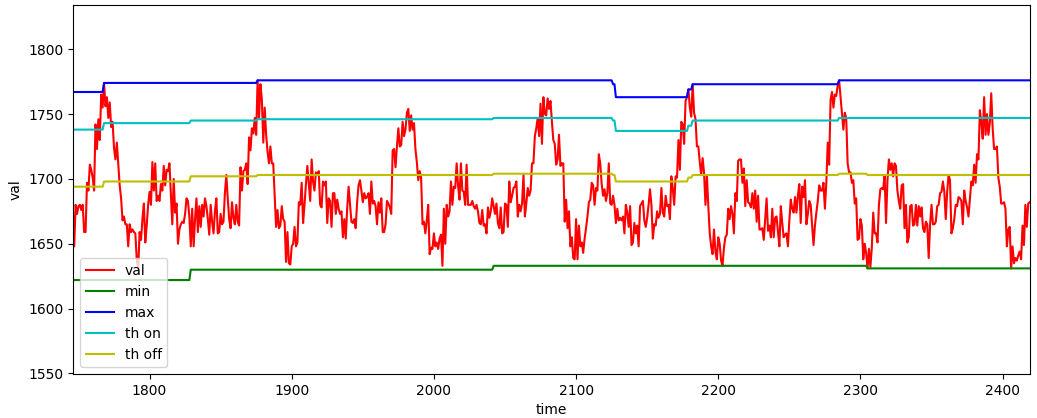
\includegraphics[width=1\textwidth]{Images/heartbeatGraph.png}
    \end{figure}

Una volta rilevati i singoli battiti con il modello matematico, il calcolo del battiti al minuto è stato realizzato salvando la cronologia degli istanti di tempo per gli ultimi N battiti $N_{beats}$. Sperimentalmente si è optato per 30 registrazioni per mantenere il valore dei bpm reattivo ma non dipendente solo da poche unità. Prelevando dalla cronologia il tempo passato $T_{diff}$ per questi battiti, si può facilmente derivare il rateo di $bpm$ attuale tramite la formula: 
\begin{equation}
bpm = \frac{ N_{beats}*60 s/min }{T_{diff}} = \frac{ N_{beats}*60 s/min }{T_{last}-T_{first}} 
\end{equation}
Il battito cardiaco risultante viene poi inviato periodicamente al Database e, qualora ci fossero anomalie, una notifica viene invece generata e inviata immediatamente.

\section{Raspberry}
Il raspberry è stato scelto come board per la computazione delle immagini di video-sorveglianza. 
Il principale concorrente a questa scelta, l'ESP32-CAM è stato testato per lo streaming video ma non è provvisto delle risorse computazionali necessarie per il rilevamento di anomalie. 
Avendo un costo inferiore rispetto al Raspberry è stato comunque considerato come alternativa low-cost. 
Il motion detector base è stato costruito come segue:
Accumulating the weighted average of the previous N frames
Taking the current frame and subtracting it from the weighted average of frames
Thresholding the output of the subtraction to highlight the regions with substantial differences in pixel values (“white” for foreground and “black” for background)
Applying basic image processing techniques such as erosions and dilations to remove noise
Utilizing contour detection to extract the regions containing motion

\section{Web App}

    
    La \textbf{Web App} è stata sviluppata come un prototipo funzionante, ma che per essere considerato completo richiederebbe ancora lavoro di rifinitura.
    
    \subsection{Considerazioni tecnologiche}
    
        L'applicazione è stata sviluppata utilizzando \textbf{nodeJS} e \textbf{VueJS}. 
        Una scelta guidata dalla semplicità del framework javascript, che a differenza di \textbf{React} e \textbf{Angular} offre una curva di apprendimento ben più bassa, favorendo lo sviluppo. 
        \textbf{VueJS} forniva inoltre il vantaggio di integrarsi perfettamente con AWS \textbf{Amplify}, a livello di \textbf{front-end}.
        Mentre a livello di \textbf{back-end} le comunicazioni sono perfettamente supportate dato che anche l'applicativo \textbf{back-end} è stato sviluppato anch'esso \textbf{nodeJS}.
        
        Il comparto estetico è sviluppato utilizzato \textbf{Vuetify} un estensione di \textbf{VueJS} che sembrava integrarsi meglio con il framework rispetto a \textbf{BootstrapVue}.
        
        Per la comunicazione con le API \textbf{REST} si è scelto di utilizzare \textbf{AXIOS} rispetto ad \textbf{AJAX} questo perche risulta di facile integrazione con \textbf{VueJS}, supporta le \textbf{SPA} e consente il facile utilizzo di \texttt{Async} e \texttt{Await}.
        
        Mentre per le \texttt{websocket} si è scelto di usare le librerie di default, principalmente per la loro semplicità di utilizzo, è stata valutata l'adozione  \texttt{Socket.io} che forniva maggiori funzionalità  e supporto a comunicazioni   come l'utilizzo di \texttt{fall back}.
        Tali funzionalità però per un uso base non erano utili è quindi stata accantonata.
        
        Per le rotte della pagina è stato utilizzato \textbf{VueRouter}
        essendo l'unica alternativa.
        
        Infine per facilitare lo sviluppo è stato utilizzato \textbf{Vuex} che consente di accedere da più punti ad un'oggetto condiviso.
        
    \subsection{Note sull'codice}
        Per questini di velocità e leggibilità si è diciso di dividere l'applicativo su più \texttt{view} : \textbf{Home} e \textbf{Login}.
        
        Ogni \texttt{view} è composta da più componenti che a loro volta sono composti.
        
        Tutti gli elementi di \textbf{VueJS} sono stati strutturati seguendo il modello del \textbf{Single File Components} che prevede di inserire il codice per lo \textbf{Style}(CSS), \textbf{Markup}(Vue/HTML) e \textbf{Script}(JavaScript) tutto nello stesso file.
        
    \subsection{Difficoltà durante lo sviluppo}
    
        Lo sviluppo della \textbf{Web App}  è stato fluido fino all'integrazione delle prima chiamata alle \textbf{API}, qui ci siamo resi conto che le api non potevano essere chiamate direttamente dal \textbf{Broswer}.
        Mentre funzionavano perfettamente utilizzando sistemi come \textbf{Postman} e \textbf{Reqbin}. 
        
        L'errore \textbf{Cross-Origin Resource Sharing} (CORS), riguarda la possibilità di utilizzare altre sorgenti per attingere informazioni, questo genere di verifica è effettuata solo dal Broswer ed è invece saltata su Postman e simili.
        
        Dopo un investigazione siamo giunti alla conclusione che in fase di \textbf{sviluppo} avremmo potuto consentire ogni richiesta. Abbiamo quindi aggiunto le seguenti linee di codice nel file \texttt{Template.yaml} di \textbf{SAM}, questo per istruire il proxy cors di AWS a rispondere alle richieste con i campi aggiunti:
        \begin{lstlisting}
        Globals:
          Api:
            EndpointConfiguration: REGIONAL
            Cors:
              AllowMethods: "'*'"
              AllowHeaders: "'*'"
              AllowOrigin: "'*'"
        \end{lstlisting}
        
        L'errore smise di apparire, ma con la necessità di testare sempre più funzioni e l'impossibilità effettuare il deploy di sam per ogni prova, abbiamo iniziato ad eseguire una istanza di AWS \textbf{Lambda} localmente tramite il comando : \texttt{sam build \&\& sam local start-api}.
        
        Giunti a questo punto il problema si è ripresentato e questa volta la soluzione è stata molto più ostica da trovare.
        Nonostante il problema fosse lo stesso e che quindi mancasse la risposta \textbf{CORS}.

        %CORS LATO BROSWER
        \begin{figure}[H]
            \caption{Errore lato Broswer}
            \label{fig:ErrorCorsBroswer}
            \centering
            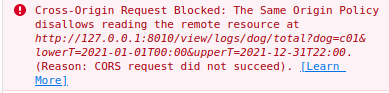
\includegraphics[width=1\textwidth]{Images/CorsErrorFrontEnd.PNG}
        \end{figure}
        
        %CORS LATO CONSOLE
        \begin{figure}[H]
            \caption{Errore lato console}
            \label{fig:ErrorCorsConsole}
            \centering
            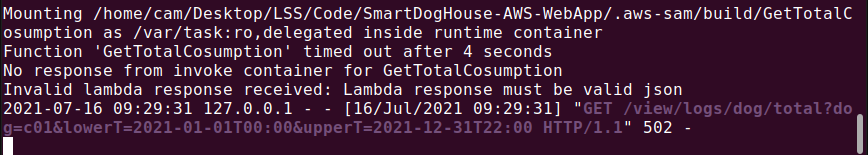
\includegraphics[width=1\textwidth]{Images/CorsErrorConsole.PNG}
        \end{figure}
    
        Volenterosi di utilizzare e testare le funzioni lambda localmente abbiamo cercato una soluzione in maniera esaustiva,
        giunti finalmente \href{https://github.com/aws/aws-sam-cli/issues/323#issuecomment-483650280}{Issue} che ha fornito la soluzione se pur non ottimale.
        
        Il comando utilizzato: \texttt{npx lcp --proxyUrl http://localhost:3000/}
        
        La soluzione adottata consiste nell'avviare un server proxy CORS che risponda alle richieste \textbf{OPTIONS} e poi reindirizzi all'immagine docker di lambda. 
        Ovviamente la WebApp dovra contattare il proxy e non direttamente il container.
        
        Nonostante gli sviluppatori di SAM confermino il supporto alle chiamate CORS locali non siamo riusciti a farle funzionare in altra maniera.
        
\subsection{Deployment} 
        Il repository è stato collegato e configurato per il continuous deploymnet, così da pubblicare e rilasciare le modifiche online non appena rilasciate se il sito compila, il sito essendo pubblico è stato protetto da password grazie ad amplify.
        
        
\section{Funzioni Serverless}
    Le principali difficoltà in questa parte del progetto sono legate all'apprendimento delle tecnologie \textbf{AWS} utilizzate,
    quali:
    \begin{itemize}
        \item \textbf{Lambda} I due principali problemi incontrati sono stati:
         \begin{itemize}
             \item Lo sviluppo e il testing in locale che richiede l'ausilio della \textbf{SAM CLI} e della \textbf{AWS CLI}.
             \item L'utilizzo del sdk di AWS per javascript sopratutto quando era necessario contattare altri servizi come IoT Core o API Gateways.
         \end{itemize}

        \item \textbf{IoT Core} Non sono stati riscontrate particolari difficolta se non con i certificati che non sono in un formato compatibile con la libreria \texttt{Umqtt} di micropython.
        \item \textbf{CloudWatch} Consultare i log delle funzioni lambda non risulta complicato, stesso non si può dire per i log delle websocket.
        \item \textbf{IAM} Il sistema dei permessi di AWS è molto articolato e ci sono più modi per fornire i permessi, in generale la gestione dei permessi è stata faticosa. Alcuni permessi sono molto immediati, altri come quello per consultare i log di \textbf{CloudWatch} delle websocket molto meno, non tanto per i permessi più per il tool grafico o la sintassi di SAM.
        \item \textbf{API gateway} L'esposizione delle \texttt{API} \textbf{REST} e delle web socket non è stata difficoltosa.
        \item \textbf{SAM} Forse la parte più complicata dell'applicativo serverless, fornisce la possibilità di effettuare il deploy di \textbf{Stack} su \textbf{AWS CloudFormation}, con una sintassi tutta sua, orchestrare il deploy di : Funzioni Lambda, Regole IoT Core, Permessi IAM, Tabelle DynamoDB, API REST, Websocket e CloudWatch Event via crono. Nonostante il grande sforzo per sfruttare al meglio SAM, il lavoro potrebbe essere ulteriormente automatizzato e perfezionato. 
    \end{itemize}
    
\subsection{Deployment} 
        L'intero stack che esclude il database principale, Aws Aplify e i dispositivi IOT può essere dispiegato tramite il comando \texttt{sam build \&\& sam deploy}
        Attualmente il deploy è dipendente da alcune variabili che sono configurabili con il flag \texttt{-g}, altre variabili sono incorporate e potrebbero essere scorporate alla stessa maniera se si volesse rendere il deploy multi-account.
        
\section{Database DynamoDB}
        Lo sviluppo del database è una parte critica del progetto,
        in un ottica di rendere l'applicativo veloce e scalabile il più possibile, abbiamo scelto di procedere con lo sviluppo di una tabella DynamoDB.
        DynamoDB offre una scalabilità e una velocità di interrogazione superiori ai database relazionali, per questo lo abbiamo scelto, inoltre la sua prefetta integrazione con il \textbf{back-end} lo rendeva ancora più appetibile.
        
        Le difficoltà durante lo sviluppo del database sono state enormi.
        Partendo dalla documentazione e dalle guide che siamo riusciti a reperire, subito ci siamo trovati in difficoltà con il mindset necessario allo sviluppo del database, troppo legati all'ambito relazionale.
        Il database ha passato molti \textbf{schemi} diversi che sono stati raffinati mano a mano che la complessità e i meccanismi del DB venivano compresi.
        Questo comportava continue modifiche al DB e il testare e studiare sono diventati essenziali, motivo per cui abbiamo scelto di non includerlo all'interno del deploy \textbf{SAM}, non si voleva complicare il complicato.
        
\subsection{Tool utilizzati}
    Durante lo sviluppo abbiamo utilizzato due strimenti per aiutarci aiutatrci nella comprensione e nello sviluppo del sistema:
    \begin{itemize}
        \item \textbf{NoSQL Workbench} Il nuovo tool grafico di AWS ci ha permesso di visualizzare con maggiore chiarezza il database e di elaborare le query utilizzando \textbf{PartiQL}.
        Inoltre ci ha anche permesso di effettuare la creazione di tabelle utilizzando la connessione ad AWS.
    \end{itemize}\textbf{PartiQL} Una gradita sorpresa durante lo studi e lo sviluppo del database. Infatti questo consente di interrogare \textbf{DynamoDB} utilizzando la classica sintassi \textbf{SQL}, molto più espressiva dell'\textbf{SDK} javascript.
    Purtroppo l'implementazione al supporto \textbf{PartiQL} non è supportata totalmente e quindi grossa parte della sintassi \textbf{SQL}
    come proiezioni e query annidate non sono disponibili.
    Questo rende l'implementazione delle query più frammentata, e ci ha obbligato a riscrivere varie parti di codice e DB.
    Tali limiti sono intrinseci di DynamoDB e non una mancaza di sviluppo parziale.

\begin{tcolorbox}[tab2,tabularx={c||c|c|Y|Y},title=Confronto Prestazioni Microcontrollori Testati,boxrule=0.5pt] \hline
board & velocità processore & costo & tempo medio avvio programma & tempo medio connessione MQTT \\ \hline
\hyperlink{https://en.wikipedia.org/wiki/ESP8266}{ESP8266} & 160 MHz & 5€ & 8,1 s & 9,3 s\\ \hline
\hyperlink{https://en.wikipedia.org/wiki/ESP32}{ESP32} & 240 MHz (dual core) & 7€ & 5,2 s & 3,4 s\\ \hline
\end{tcolorbox}

\input{Tex/Implementation/SaraKiade}
\input{Tex/Implementation/GyordanCaminati}
